\chapter{Knoxly, un tool di privacy awareness}
Una volta implementato il core basato su Intelligenza Artificiale, in questo capitolo parliamo di come è stato sviluppato ed aggiornato il tool Knoxly.
 
Nella Sezione~\ref{sec:whoisKnoxly} sono stati spiegati il funzionamento, gli obiettivi e i limiti del progetto Knoxly, una estensione per Google Chrome volta a fornire privacy awareness agli utenti riguardo il contenuto dei messaggi che sono in procinto di pubblicare sul Web. Prima di questo lavoro Knoxly era in grado di segnalare all'utente la presenza di dati sensibili e/o personali presenti in un testo scritto in italiano o inglese basandosi su un analizzatore lessicale (quindi utilizzando una logica keyword-based). Ora Knoxly può contare su una analisi del testo migliore dato che adesso è dotato di tre moduli: (a) il \textit{Topic classifier} (Sez~\ref{sec:topicclass}) che è in grado di capire a quale fra cinque topic (politics, health, job, travel e general) appartiene un testo scritto in una tra 16 lingue (vedi Sezione~\ref{sec:use}), (b) il \textit{Sensitivity classifier} (Sezione~\ref{sec:sensclass}) che è in grado di comprendere quanto un testo sia sensibile o meno (sempre in 16 lingue) e (c) il \textit{Customized sensitivity classifier} (Sezione~\ref{sec:pres_sens_class}) che è in grado apprendere le preferenze degli utenti in fatto di privacy e regolare le segnalazioni di Knoxly di conseguenza.

Più nello specifico, in questo capitolo si mostra il flusso di lavoro di Knoxly (Sezione~\ref{sec:workflow}), il client-side con la User Interface (UI) (Sezione~\ref{sec:frontend}) e il server-side (Sezione~\ref{sec:backend}).

\section{Workflow}
\label{sec:workflow}
In questa sezione si descrivono i vari step che affronta un testo scritto in linguaggio naturale analizzato da Knoxly. In figura~\ref{fig:workflow} è presente una illustrazione del flusso di lavoro del tool e di come le varie componenti interagiscono tra loro.

\begin{figure}[h]
    \centering
    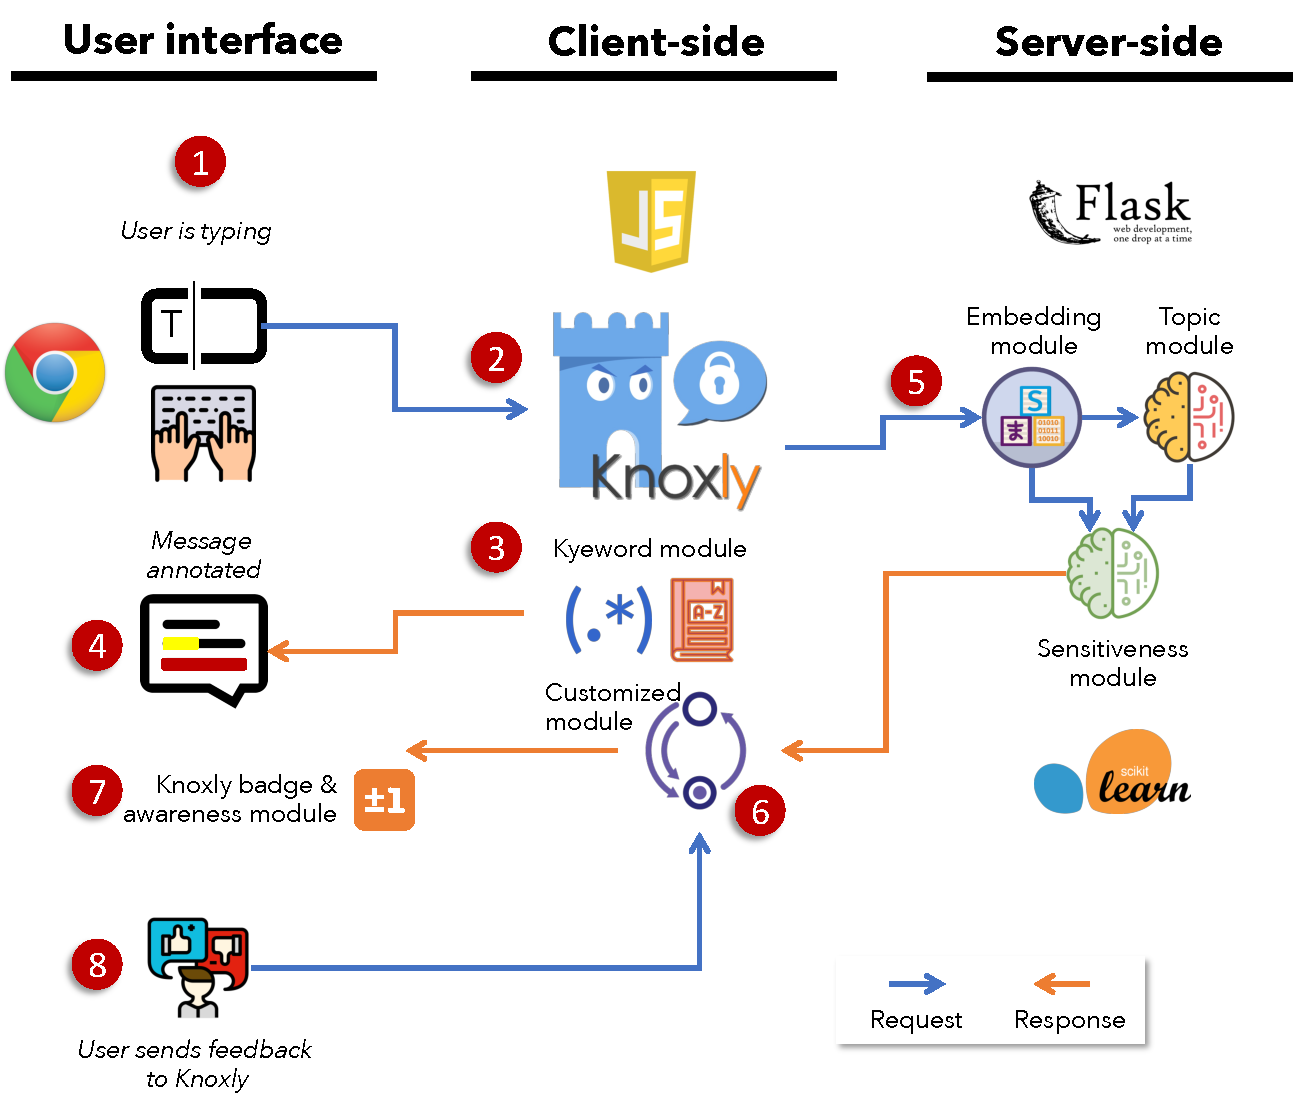
\includegraphics[width=15cm]{Figure/workflow.pdf}
    \caption{schema riassuntivo del workflow di Knoxly}
    \label{fig:workflow}
\end{figure}
\FloatBarrier
L'interazione che un utente ha con Knoxly avviene nel seguente modo:
\begin{enumerate}
    \item L'utente digita un testo $t$;
    \item Il testo $t$ viene inviato al plug-in Knoxly;
    \item $t$ viene innanzitutto analizzato con il \textit{Keyword module} utilizzando espressioni regolari e dizionari (codificati in Knoxly);
    \item Le keyword in $t$ che hanno una corrispondenza con le espressioni regolari o con i dizionari vengono evidenziate con l'ausilio di un tag {\tt <span>} a cui è associata una opportuna classe {\tt .css} (\textit{giallo} per i quasi identifier~\cite{quasiID} e dati sensibili, \textit{rosso} per i dati personali). Si fornisce inoltre la possibilità di anonimizzare le keyword segnalate utilizzando la k-anonimity~\cite{kAnonimity} (qui termina l' analisi lessicale);
    \item Knoxly invia $t$ al server Flask\footnote{https://flask.palletsprojects.com/en/1.1.x/} il quale effettua l'embedding della frase tramite l'embedding module (basato su multilingual Universal Sentence Encoder), dopidichè invia l'embed al \textit{Topic module} ed al \textit{Sensitiveness module}. Il Topic module, basato sul Topic classifier, stabilisce a quale topic appartiene $t$. In base a questo si richiama l'opportuno \textit{Sensitiveness Classifier} nel \textit{Sensitiveness module}. Quest'ultimo restituisce un vettore di due elementi (sensibilità negativa e sensibilità positiva), percentuale delle classi,  il quale, insieme all'embed verranno restituiti al client-side.
    \item Il server invia al client un vettore di 514 elementi ovvero l'embed (512 elementi) con accodatio il vettore della probabilità delle classi (2 elementi) restituito dal \textit{Sensitiveness module}. Questa risposta viene elaborata dal \textit{Customized sensitiveness module}, il quale (a) la smista al \textit{Customized Sensitiveness classifier} adatto a quel topic, (b) valuta se il contenuto risulta sensibile secondo la percezione della privacy che ha l'utente.
    \item Se il \textit{Customized Sensitiveness classifier} classifica il contenuto restituitogli dal server come sensibile, cioè un contenuto che rappresenta una minaccia alla privacy dell'utente, allora lo segnala all'utente incrementando un contatore numerico posto in un badge dell'icona di Knoxly in Google Chrome, oltre ad aggiungerlo in una list box - progettata per fornire awareness - consultabile aprendo il popup del tool.
    \item L'utente ha la possibilità di cliccare su di un bottone \quotes{feedback} indicando a Knoxly di evitare di segnalare (come sensibili) in futuro quel tipo di testi. Tale operazione aggiorna i pesi del \textit{Customized Sensitiveness Classifier} di riferimento per i testi appartenenti a quel topic.
\end{enumerate}

\section{Client-side}
\label{sec:frontend}
In questa sezione si dettagliano le caratteristiche del lato client di Knoxly.

\subsection{Euristica di input}
\label{ssec:euristicInput}
Uno dei problemi affrontati in fase di sviluppo è comprendere quando è più opportuno chiamare i moduli basati su intelligenza artificiale di Knoxly. È evidente che l'utilizzo smisurato di moduli del backend risulterebbe in un appesantimento del servizio, rendendolo lento, fastidioso e inutilizzabile. Inoltre ciò comporterebbe l'analisi di testi che non rappresentano vere e proprie frasi, cioè composte da almeno \textit{soggetto}, \textit{predicato} e \textit{complemento}, o comunque che includono un numero tale di parole da poterne comprendere la semantica. Quindi, in altri termini, la domanda è\textit{ "quando è il momento adatto per inviare una frase al server e quando invece bisogna solo affidarsi al Keyword module?"}.

Per rispondere a questo quesito bisogna definire una \textit{euristica di input} che deve garantire l'invio di frasi verso il server di Knoxly senza rischiare di creare un collo di bottiglia. 

L'euristica di input è stata definita come segue: sia $txt$ il vettore contenente i caratteri che l'utente ha digitato, $n$ la lunghezza del vettore $txt$, $txt[last]$ l'ultimo carattere presente in $txt$ e $T = \{".", ";", "!", "?"\}$ l'insieme dei caratteri che vengono posti alla fine di una frase scritta in linguaggio naturale, allora
$$ n>=5 \And txt[last] = x \in T \implies \text{invia txt al server}$$.
L'invio della frase al server avviene tramite una chiamata {\tt AJAX} verso l'endpoint del server di Knoxly. Quando arriva la risposta dal server viene chiamato il \textit{Customized Sensitiveness module} per valutare se il testo risulta sensibile anche sulla base della percezione di privacy che ha l'utente.

\subsection{User Interface per fornire privacy awareness}
\label{ssec:ui}


La User Interface (UI) di Knoxly è stata progettata ed implementata per fornire privacy awareness in modo semplice ed intuitivo. Come anticipato in Sezione~\ref{sec:whoisKnoxly} Knoxly evidenzia contenuti sensibili e/o personali presenti in un testo scritto in italiano o in inglese tramite l'utilizzo di espressioni regolari e dizionari. Utilizziamo il \textit{giallo} per i quasi identifier~\cite{} e dati sensibili, il \textit{rosso} per i dati personali. 

Cliccando sull'icona posta accanto alla barra dell'indirizzo su Google Chrome, viene visualizzato il popup di Knoxly. Accanto all'icona è possibile inoltre visualizzare un badge che riporta un contatore numerico (vedi Figura~\ref{fig:uiKnoxly}). Tale contatore è utilizzato per segnalare all'utente il numero di frasi scritte classificate come minacce per la sua privacy, cioè sensibili. 


\begin{figure}[h]
    \centering
    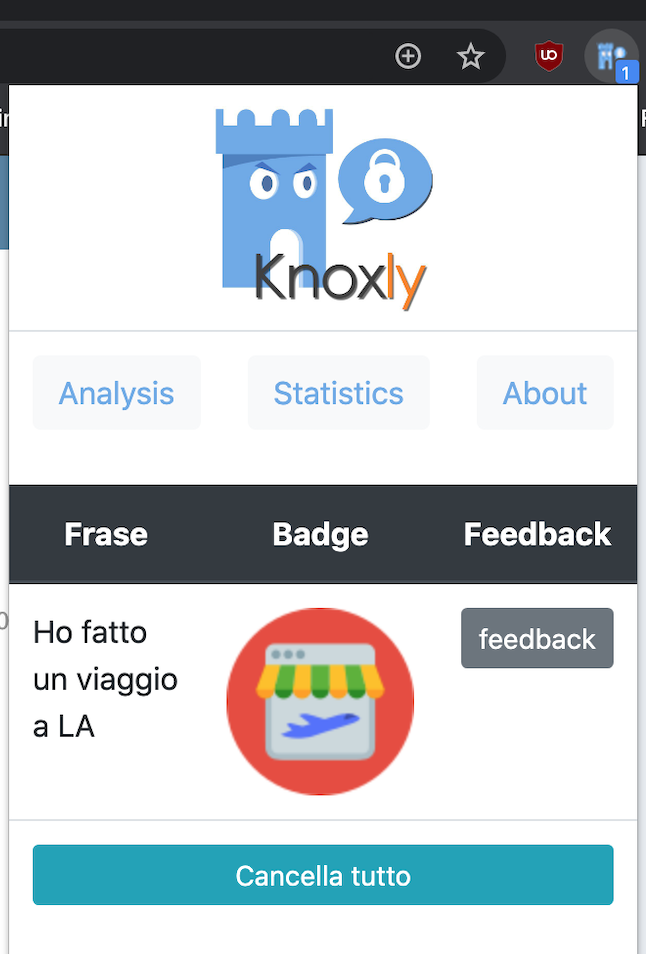
\includegraphics[scale=0.7]{Figure/ui/UI-Knoxly.png}
    \caption{User Interface di Knoxly}
    \label{fig:uiKnoxly}
\end{figure}
\FloatBarrier

In Figura~\ref{fig:uiKnoxly} viene mostrata la landing page una volta aperto il popup di Knoxly. La UI del popup è composta principalmente da tre sezioni/pagine:
\begin{itemize}
    \item \textbf{Analysis}: pagina dedicata alle segnalazioni del tool. La pagina fa anche da landing page;
    \item \textbf{Statistics}: pagina dedicata alle misurazioni, utili a rendere l'utente consapevole di ciò che scrive e quanto;
    \item \textbf{About}: pagina dedicata ad istruzioni sull'utilizzo di Knoxly.
\end{itemize}

\textbf{Analysis} è composta da una tabella con tre colonne. Mostra le frasi che Knoxly reputa sensibili, indicando una icona facente riferimento al topic a cui appartiene la frase che può avere due colori: \textit{giallo} nel caso in cui la frase risulti sensibile (sensibilità positiva compresa fra $0.36$ e $0.68$) o \textit{rosso} nel caso in cui la frase abbia una sensibilità positiva maggiore o uguale a $0.68$. Inoltre viene mostrato anche il bottone \textbf{feedback} che consente all'utente di inviare un feedback a Knoxly per far si che il tool non segnali più come sensibili frasi simili a quella per cui si sta inviando il feedback.

Le icone scelte per fornire consapevolezza sono mostrate in Figura~\ref{fig:bollini}. Sono stati utilizzati i colori \textit{rosso} e \textit{giallo}, in quanto il colore rosso è il colore maggiormente utilizzato per definire un pericolo/rischio, mentre, il colore giallo è il colore maggiormente utilizzato per definire l'avviso\quotes{avviso}.
\begin{figure}[h!t]
    \centering
    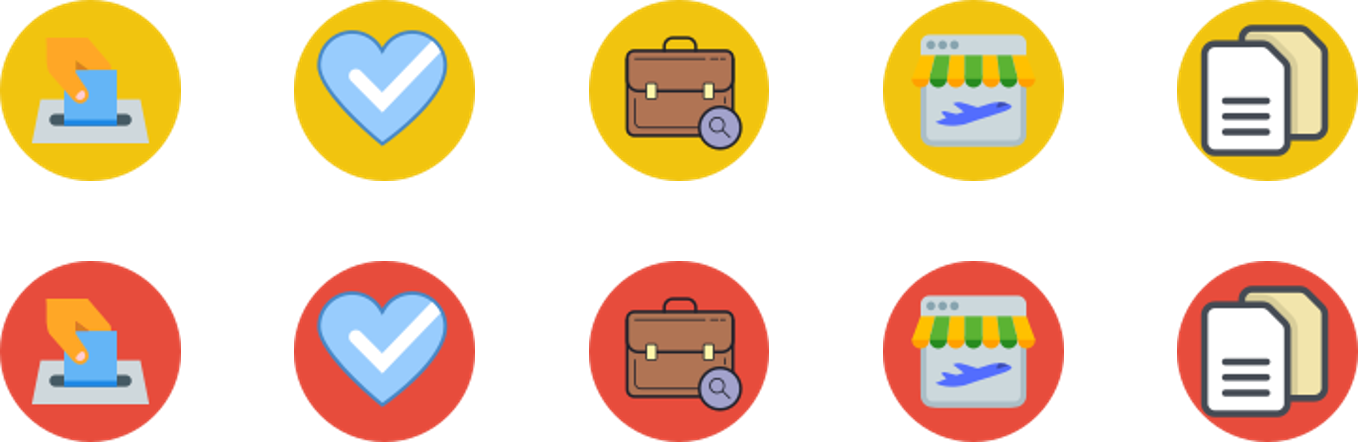
\includegraphics[scale=0.7]{Figure/ui/bollini.png}
    \caption{icone presenti in Knoxly}
    \label{fig:bollini}
\end{figure}
\FloatBarrier


La sezione \textbf{Statistics} (vedi Figura~\ref{fig:statKnoxly}) è dedicata alle misurazioni: l'utente può visualizzare un grafico a barre che riporta il numero di occorrenze di frasi sensibili che lui ha divulgato in rete nei vari topic, politica, salute, viaggi, lavoro e general. Al di sotto del grafico a barre l'utente può visualizzare l'\textbf{overall score} della sensibilità dei contenuti che divulga in rete. L'overall score $s$ viene calcolato come la media aritmetica delle sensibilità date alle frasi ritenute sensibili da Knoxly.

L'overall score non è altro che il calcolo online della media degli score di sensibilità ottenuti per ciascuna delle frasi che ha divulgato, con riferimento alle sole frasi classificate sensibili. Lo score $s \in [0..1]$ e viene rappresentato come un cerchio che si colora di rosso se l'overall score supera 0.68 altrimenti è mostrato in giallo. 
\begin{figure}[h]
    \centering
    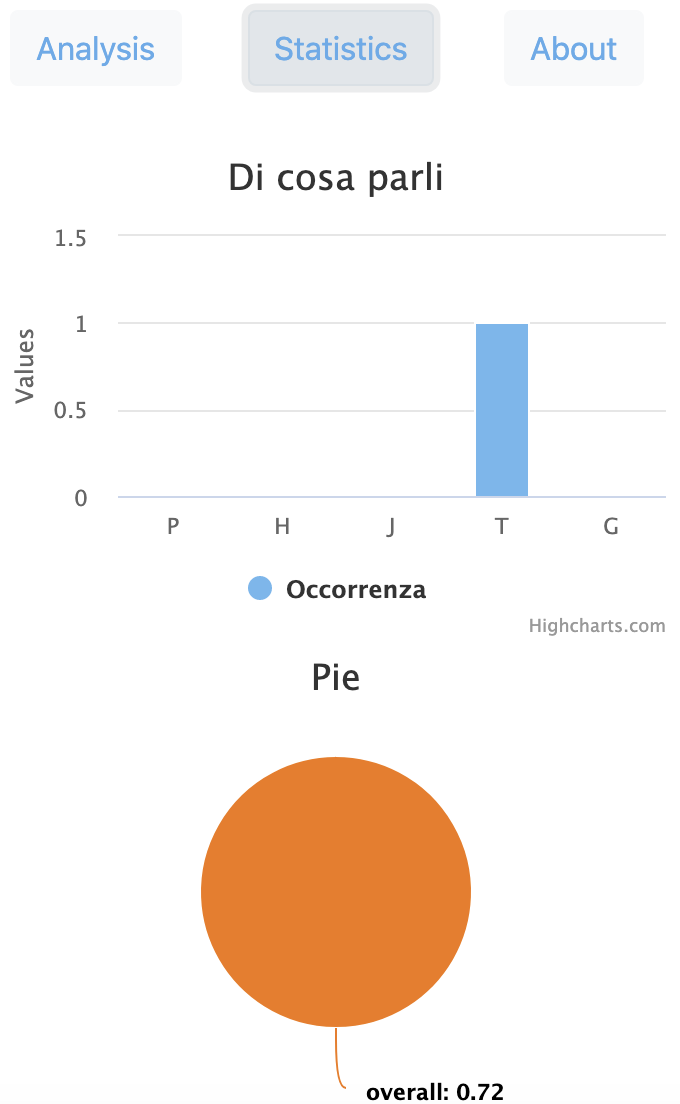
\includegraphics[scale=0.7]{Figure/ui/statistics.png}
    \caption{sezione statistics di Knoxly}
    \label{fig:statKnoxly}
\end{figure}
\FloatBarrier

Infine nella sezione \textbf{About} (vedi Figura \ref{fig:about}) vengono riportate le informazioni riguardanti le metafore visuali adottate, con particolare focus sulle icone utilizzate per ciascun topic.

\begin{figure}[h]
    \centering
    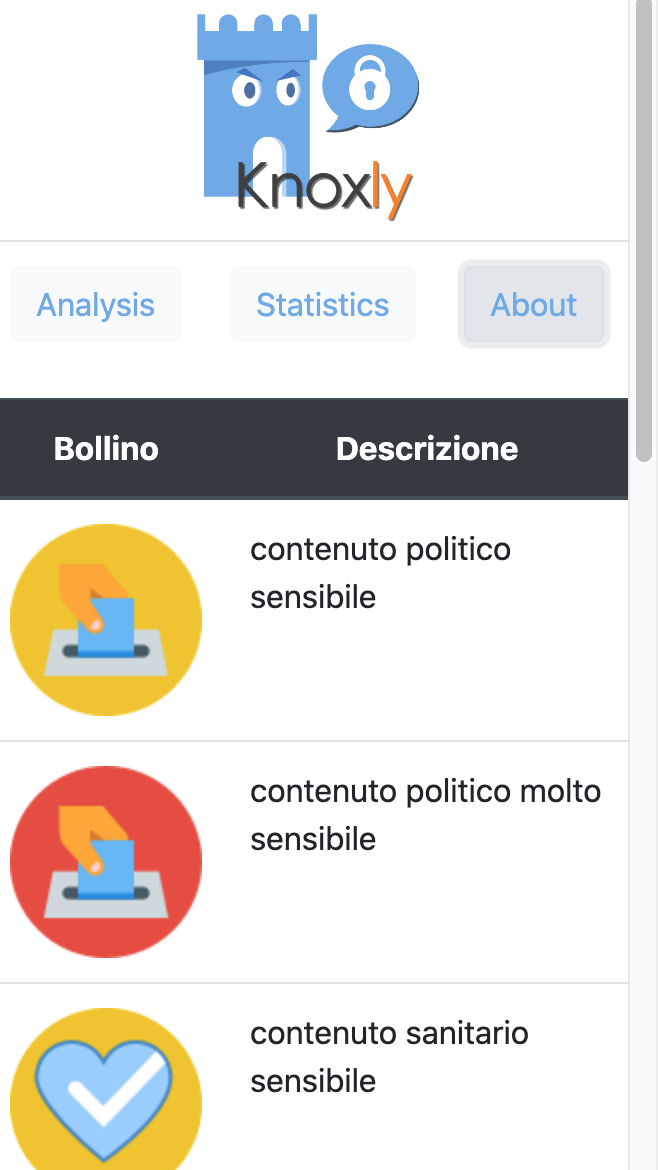
\includegraphics[scale=0.7]{Figure/ui/about.png}
    \caption{sezione about di Knoxly}
    \label{fig:about}
\end{figure}
\FloatBarrier

La UI di Knoxly è stata realizzata utilizzando Bootstrap\footnote{\url{https://getbootstrap.com/}}, e Highcharts\footnote{\url{https://www.highcharts.com/}} per i grafici.

\section{Server-side}
\label{sec:backend}
Il lato server di Knoxly è molto semplice: esso è stato realizzato in Flask\footnote{\url{https://flask.palletsprojects.com/en/1.1.x/}} ed è composto da un unico end point. Quest'ultimo riceve il testo dal client, effettua l'embed utilizzando mUSE, chiama il Topic classifier e in base al topic individuato chiama il Sensitiveness classifier di competenza, dopodichè invia l'embed con accodato il vettore contenente la sensibilità negativa e positiva al client affichè questo possa valutare se la frase risulta sensibile anche per la percezione di privacy che ha l'utente.